\section{Liczba kolorująca}
    \subsection{Co to w ogóle jest}
    Liczba kolorująca jest źródłem konfuzji dla niezliczonych studentów. Co ona w ogóle robi, po co jest i dlaczego nie ma jej w żadnej literaturze? Na to ostatnie pytanie nie odpowiem, ale liczba kolorująca, oznaczana również jako $col(G)$ jest użyteczna, bo, jak za niedługo pokażemy, ogranicza od góry $\chi(G)$ oraz da się ją obliczyć w czasie wielomianowym (na wypadek gdyby ktoś się jeszcze nie zorientował, kolorowanie grafów jest problemem klasy NP-przykrej). Poza tym jestem zdania, że nazwanie tego \textit{liczba kolorująca} to fatalna decyzja, bo dosyć ładnie kamufluje co to w ogóle jest; w tym momencie chciałbym napisać coś śmiesznego o matematykach i dziwnych decyzjach, ale nic śmiesznego nie przychodzi mi do głowy. 
    \subsubsection{Definicja}
    Rozpatrzmy wszystkie permutacje wierzchołków grafu $G$. Zdefiniujmy funkcję $f$, która dla każdego wierzchołka w obrębie danej permutacji przypisuje liczbę jego sąsiadów, którzy wystąpili ,,przed nim'' w permutacji. Zdefiniujmy funkcję $g$, która dla danej permutacji wynosi maksymalnej wartości funkcji $f$ policzonej dla wszystkich wierzchołków z tej permutacji i dodaje do tego jeden. Skąd wytrzasnęła się ta jedynka zaraz się dowiemy, obiecuję że to nie jest kolejny arbitralny wymysł matematyków którzy wypili za dużo kawy (tak jak nazwa tego bytu).  

    Fajnie teraz zauważyć, że $g$ dla danej permutacji oszacowuje z góry jak bardzo może ,,skopać'' kolorowanie algorytm First-Fit, jeśli pokoloruje wierzchołki zgodnie z tą permutacją; w najgorszym przypadku, gdy istnieje jakiś wierzchołek mający $d$ sąsiadów ,,na lewo'' i wszyscy mają różne kolory, to FF da mu kolor $d+1$. Stąd maksymalna liczba sąsiadów na lewo wśród wierzchołków ($+1$) daje nam górne oszacowanie na to, jak First-Fit może popsuć kolorowanie \textit{jeśli będzie kolorować według tej permutacji}.  

    Nikogo teraz chyba nie zdziwi fakt, że $col(G)$ to jest po prostu minimum po funkcjach $g$ dla wszystkich permutacji wierzchołków grafu $G$. 
    \subsection{Relacja z liczbą chromatyczną}
    \subsubsection{Ograniczenie liczby chromatycznej przez liczbę kolorującą}
    \begin{theorem}[Relacja liczby kolorującej z liczbą chromatyczną]
        \begin{equation}
            \chi(G) \leq col(G)
        \end{equation}
    \end{theorem}
    \begin{proof}
        Gdy tak nie było, to istniałaby taka permutacja wierzchołków grafu że First-Fit pokolorowałby graf lepiej niż $\chi(G)$ mówi, że da się pokolorować. Koniec dowodu. Serio.
    \end{proof}
    \subsubsection{Ograniczenie liczby kolorującej przez jakąś funkcję liczby chromatycznej}
    Nie da się. Znaczy da się, ale tylko w pewnych klasach grafów. W ogólnej klasie grafów istnieją takie grafy, że liczba kolorująca leci do nieskończoności, a $\chi(G) = 2$. Grafem takim jest na przykład klika dwudzielna $K_{n,n}$. Swoją drogą to jest protip: jeśli potrzebujesz udowodnić że $col(G)$ nie da się ograniczyć w jakiejś klasie grafów przez funkcję $\chi(G)$, spróbuj pokazać że da się tam skonstruować klikę dwudzielną. Nie ma za co. 
    \subsection{Algorytm obliczania liczby kolorującej}
        \begin{theorem}[Magiczny wzór na liczbę kolorującą]
            \begin{equation}
                col(G) = \mathrm{max}\{ \delta(H) : H \subset_{ind.} G \} + 1
            \end{equation}
        \end{theorem}

        \begin{proof}
            Ten wzór wygląda na początku dziwnie, ale w sumie ma sens. Dowodzić to będziemy trochę dziwnie, bo zamiast pokazywać od razu równość, pokażemy ograniczenie z góry i z dołu (skąd będziemy mieć, że istotnie zachodzi równość). 

            Pokażmy zatem nierówność w pierwszą stronę:
               \begin{equation*}
                    col(G) \geq \mathrm{max}\{ \delta(H) : H \subset_{ind.} G \} + 1
               \end{equation*}

            Dowód jest dosyć prosty; jeśli $col(G) = k$ dla jakiegoś $k$, to znaczy to że istnieje jakaś permutacja wierzchołków $G$ taka, że każdy wierzchołek ,,na lewo'' ma  co najwyżej $k-1$ sąsiadów. Teraz dla każdego podgrafu indukowanego $H$ jest tak, że gdzieś w tej permutacji jest ,,ostatni'' wierzchołek należący do tego podgrafu indukowanego. Nie ma on w ogóle krawędzi ,,na prawo'' i ma same krawędzie ,,na lewo''. Minimalnie może ich mieć $\delta(H)$, czyli w takim razie $\delta(H) \leq k - 1$, skąd mamy że $k \geq \delta(H) + 1$ dla dowolnego podgrafu indukowanego (skąd mamy już tezę). 

            W drugą stronę dowód przy okazji pokazuje nam wielomianowy algorytm obliczania $col(G)$. Nie ukrywam że jest on bardzo fajny. 

                 \begin{equation*}
                    col(G) \leq \mathrm{max}\{ \delta(H) : H \subset_{ind.} G \} + 1
               \end{equation*}

            Konstruujemy sobie permutację wierzchołków grafu $G$. W jaki sposób? Bierzemy wierzchołek o najmniejszym stopniu i wrzucamy go \textit{na koniec} permutacji. Następnie rozpatrujemy podgraf indukowany $H$, bez tamtego wierzchołka o najmniejszym stopniu. $H$ znowu ma jakiś wierzchołek o minimalnym stopniu, więc dorzucam go na koniec permutacji (przed wcześniejszym wierzchołkiem o minimalnym stopniu) i kontynuuję ,,obgryzanie''. Nietrudno zauważyć, że każdy wierzchołek ma ,,na lewo'' od siebie jakieś $\delta(H)$ sąsiadów (gdzie $H$ jest jakimś podgrafem indukowanym). Tym samym col jest z pewnością mniejszy lub równy niż maksymalny minimalny stopień wierzchołka w jakimś podgrafie indukowanym ($+1$). 

            Pokazaliśmy więc, że nasz ,,algorytm'' generuje optymalną permutację, bo pokazaliśmy wcześniej że lepiej się nie da (pokazując ograniczenie dolne na $col(G)$). Jednocześnie dowodzi to równości.
        \end{proof}
        


\section{Kolorwanie krawędziowe grafów dwudzielnych}
\begin{theorem}
	Graf dwudzielny \(G\) można pokolorować krawędziowo przy użyciu \(\Delta(G)\) wierzchołków.
\end{theorem}
\begin{proof}
	Dowód przez indukcję po liczbie krawędzi; przypadek bazowy trywialny. Do poprawnie pokolorowanego grafu dwudzielnego \(G = (X,Y,E)\) dokładamy krawędź między jakimiś \(x\) i \(y\) i pokażemy, że taki graf również da się poprawnie pokolorować krawędziowo stosując \(\Delta(G)\) kolorów.

	Zauważam, że jako że krawędź między \(x \in X\) i \(y \in Y\) nie ma jeszcze koloru, to zarówno \(x\) jak i \(y\) muszą mieć jakiś kolor ,,wolny'', tzn. odpowiednio dla \(x\) jak i \(y\) muszą istnieć jakieś kolory \(\alpha, \beta\) takie, że krawędź o kolorze \(\alpha\) nie ,,wchodzi'' do \(x\), a krawędź o kolorze \(\beta\) nie ,,wchodzi'' do \(y\). Jeśli \(\alpha = \beta\) to kolorujemy krawędź między \(x\) i \(y\) na kolor \(\alpha\) no i mamy poprawne kolorowanie. Trochę nudne.

	Ciekawszy przypadek jest, gdy \(\alpha \not = \beta\): wtedy musimy jakoś sprytnie przekolorować \(G\), by móc pokolorować krawędź między \(x\) i \(y\) na jakiś kolor. Załóżmy że do \(x\) wchodzi krawędź o kolorze \(\beta\), a do \(y\) o kolorze \(\alpha\) (bo inaczej byśmy to trywialnie pokolorowali). Spójrzmy na wierzchołek z którym łączy się \(x\) krawędzią o kolorze \(\beta\); nazwijmy go \(y_1\). Zauważmy, że z \(y_1\) musi wychodzić krawędź o kolorze \(\alpha\), bo gdyby krawędź \(\alpha\) była wolna dla \(y_1\), to krawędź koloru \(\beta\) mógłbym przekolorować na kolor \(\alpha\), a więc kolor \(\beta\) w \(x\) by się ,,zwolnił'' i mógłbym przekolorować naszą oryginalną krawędź na \(\beta\), otrzymując poprawne kolorowanie spełniające tezę zadania.

	Wierzchołek z którym łączy się \(y_1\) za pomocą koloru \(\alpha\) nazwijmy zatem \(x_1\). Chyba już widzimy kierunek w którym to zmierza. \(x_1\) łączy się kolorem \(\beta\) z jakimś \(y_2\), bo jeśli nie to kolor \(\beta\) jest ,,wolny'' i możemy wcześniejszą krawędź przekolorować na niego, zwalniając jej kolor w wierzchołku \(y_1\) i umożliwiając dalsze przekolorowanie.

	Sekwencję takich wierzchołków, opisaną w ten sposób nazwiemy \(\beta\alpha-\)ścieżką. Zauważam że ścieżka ta nigdy nie może się ,,zacyklić'' w grafie dwudzielnym (w tym wrócić do \(x\) lub \(y\)) bo wygenerowałoby to sprzeczność z założeniami dotyczącymi kolorowania. Jednocześnie jako że graf jest skończony, musi ona gdzieś się skończyć. Znaczy to że dojdziemy w pewnym momencie do jakiegoś punktu, od którego będziemy mogli przekolorować całą tę ścieżkę i uzyskać poprawne kolorowanie całego grafu \(G\).
\end{proof}


\section{Twierdzenie Vizinga}
    Jest to dowód, który najłatwiej zrozumieć samemu rozrysowując sobie proces na kartce. Niemniej, z pomocą rysunków spróbuję go Wam przybliżyć.
    
    \begin{theorem}[Vizing]
        $$\Delta(G) \leq \chi'(G) \leq \Delta(G) + 1$$
    \end{theorem}
    
    \begin{proof}
        Ograniczenie dolne widzimy od razu -- $\Delta$ krawędzi spotykających się w jednym wierzchołku musi dostać różne kolory. 
        
        Ograniczenie górne pokazujemy indukcją po liczbie pokolorowanych krawędzi. Jedną krawędź umiemy pokolorować bez problemu.
        Weźmy zatem częściowe kolorowanie i powiedzmy, że chcemy pokolorować krawędź $(x, y)$.
        
        Skoro mamy do dyspozycji $\Delta + 1$ kolorów to znaczy, że każdy wierzchołek ma jakiś kolor wolny (nie wychodzi z niego krawędź w tym kolorze). 
        
        Obserwacja, z której będziemy dużo korzystać: jeśli dowolne wierzchołki $x$, $y$ połączone krawędzią mają wolny ten sam kolor $\beta$
        to krawędź między nimi możemy pokolorować na tenże kolor. Kolory wolne dla danego wierzchołka będziemy oznaczać linią przerywaną. dotykającą tego wierzchołka.
        
        \begin{figure}[ht]
            \centering
            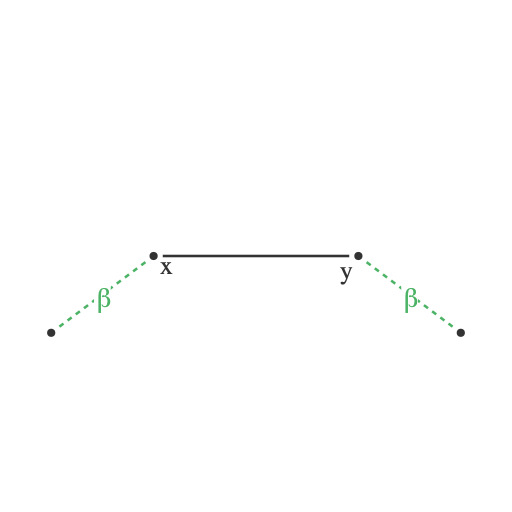
\includegraphics[scale=0.6]{chapters/dyskretna/colours/vizing/images/trivial_case.png}
            \caption{prosty przypadek; $x$ i $y$ mają wolny ten sam kolor $\beta$}
        \end{figure}
        
        Załóżmy więc, że mamy pecha i wierzchołki $x, y$ nie mają wspólnych wolnych kolorów tj. jeśli $x$ ma wolny kolor $\beta$
        to $y$ ma ten kolor zajęty i vice versa. Dodatkowo niech $\alpha_0$ będzie wolnym kolorem wierzchołka $y$.
        
        Od tego momentu będziemy tak kombinować, żeby $x$ zwolnić $\alpha_0$, być może zajmując przy tym $\beta$.
        
        \begin{figure}[H]
            \centering
            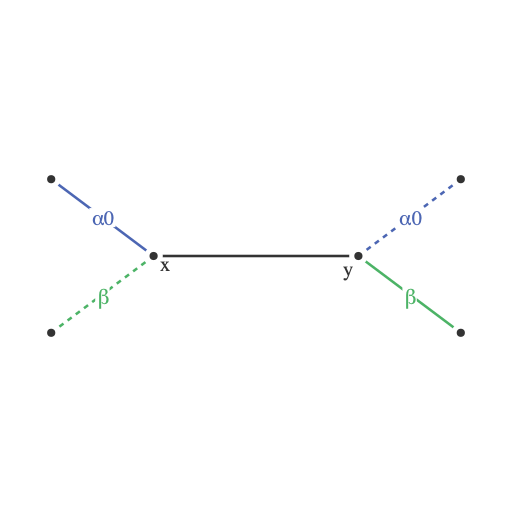
\includegraphics[scale=0.6]{chapters/dyskretna/colours/vizing/images/pre_step_one.png}
            \caption{$x$ i $y$ nie mają wspólnych wolnych kolorów}
        \end{figure}
        
        
        Niech $x_0$ będzie taki, że krawędź $(x, x_0)$ ma kolor $\alpha_0$. Jeśli $x_0$ ma wolny kolor $\beta$
        to krawędź $(x, x_0)$ możemy przekolorować na kolor $\beta$,
        tym samym sprawiając, że $x$ ma wolne $\alpha_0$.
        Ale w takiej sytuacji możemy pokolorować $(x, y)$ na kolor $\alpha_0$. 
        
        Zatem sytuacja ma się teraz tak:
        
        \begin{figure}[ht]
            \centering
            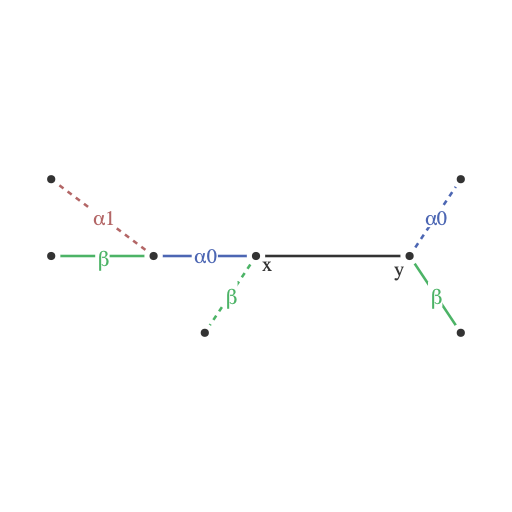
\includegraphics[scale=0.6]{chapters/dyskretna/colours/vizing/images/step_one.png}
            \caption{$x$ i $y$ mają wolne różne kolory, $x_0$ ma zajętą $\beta$ i wolne $\alpha_0$}
        \end{figure}
        
        Jeżeli teraz $x$ ma wolny kolor $\alpha_1$ to krawędź $(x, x_0)$
        możemy przekolorować na $\alpha_1$, a krawędź $(x, y)$ na $\alpha_0$. Niech więc $(x, x_1)$ będzie w kolorze $\alpha_1$.
        
        Jeśli $x_1$ miałby wolny kolor $\beta$ to możemy przekolorować $(x, x_1)$ na $\beta$, wtedy $x$ zwalnia się $\alpha_1$ a z tym wiemy co robić. 
        No to niech w $x_1$ $\beta$ będzie zajęta, a wolny będzie kolor $\alpha_2$. Poniżej ilustracja:
        
        \begin{figure}[ht]
            \centering
            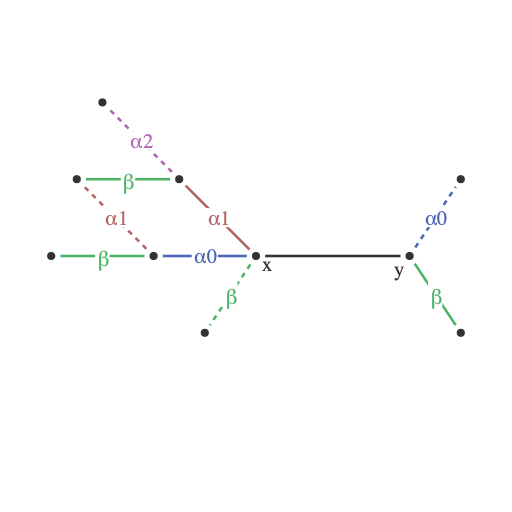
\includegraphics[scale=0.6]{chapters/dyskretna/colours/vizing/images/step_two.png}
            \caption{$x_1$ ma zajętą $\beta$ a wolne $\alpha_2$}
        \end{figure}
        
        Podobnie jak wcześniej stwierdzamy, że z $x$ wychodzi krawędź w kolorze $\alpha_2$, bo inaczej przekolorujemy $(x, x_1)$ na $\alpha_2$. Kontynuujemy to rozumowanie aż napotkamy wierzchołek $x_k$ o wolnym kolorze $\alpha_j$, który już znajduje się wśród kolorów $\alpha_0, ..., \alpha_{k-1}$
        
        
        \begin{figure}[ht]
            \centering
            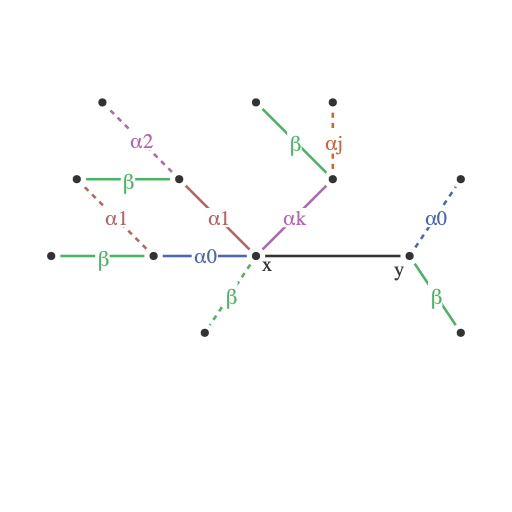
\includegraphics[scale=0.6]{chapters/dyskretna/colours/vizing/images/step_three.png}
            \caption{$x_k$ ma wolny kolor $\alpha_j$, który już widzieliśmy.}
        \end{figure}
        
        Niestety nie możemy wykonać tej samej sztuczki z przekolorowaniem co wcześniej, ale to nic nie szkodzi bo zrobimy co innego.
        Otóż wyjdźmy z wierzchołka $x_k$ i pójdźmy ścieżką w kolorach na przemian $\beta$ i $\alpha_j$.
        Oczywiście kiedyś skończą nam się krawędzie i wylądujemy w jakimś wierzchołku $v$.
        
        Rozważmy sobie teraz przypadki czym ten wierzchołek $v$ jest.
        
        \begin{enumerate}
            \item $v \notin \{x, x_0, x_1, ..., x_k\}$ 
            Najfajniejszy przypadek - ścieżka kończy się w niezbyt istotnym miejscu. Zamieniamy kolory na ścieżce miejscami. Możemy tak zrobić, bo wewnętrznym wierzchołkom się nic nie zmienia, a na końcach odpowiedni kolor jest wolny.
            
            Teraz, począwszy od krawędzi $(x, x_k)$ przekolorujemy wachlarz. 
            Dzięki przekolorowaniu, $x_k$ ma teraz wolną $\beta$ tak jak $x$, zatem $(x, x_k)$ możemy dać kolor $\beta$ 
            W takim razie $x$ ma teraz wolny kolor $\alpha_k$ tak jak $x_{k - 1}$, 
            zatem $(x, x_{k-1})$ dostanie kolor $\alpha_k$.
            Podobnie $(x, x_{k-2})$ dostanie kolor $\alpha_{k-1}$.
            
            W końcu dojdziemy do $(x, x_0)$, które dostanie kolor $\alpha_1$. Sprawiliśmy, że $x$ ma wolne $\alpha_0$,
            więc z czystym sumieniem kolorujemy $(x, y)$ na $\alpha_0$. 
            
            \begin{figure}[H]
                \centering
                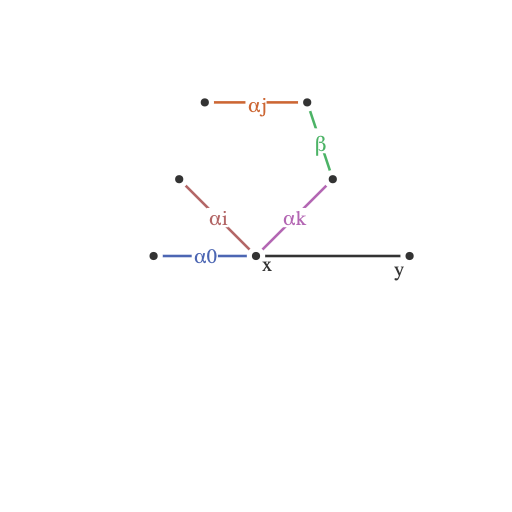
\includegraphics[scale=0.45]{chapters/dyskretna/colours/vizing/images/fan_case_one_before.png}
                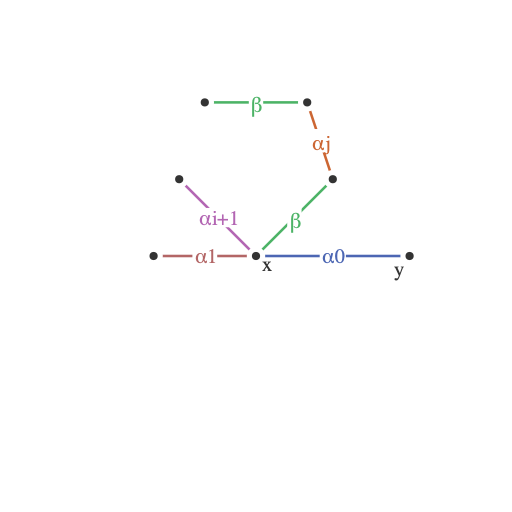
\includegraphics[scale=0.45]{chapters/dyskretna/colours/vizing/images/fan_case_one_after.png}
                \caption{Przekolorowanie wachlarza gdy ścieżka z $x_k$ kończy się w poza wierzchołkami $x, x_0, ..., x_k$}
            \end{figure}
            
            \item $v = x_{j - 1}$ 
            Taka sytuacja niestety może zajść, bo $x_{j-1}$ ma wolny kolor $x_j$ i zajętą $\beta$.
            Zauważmy, że nie możemy zrobić tego co w przypadku pierwszym, bo przekolorowanie ścieżki sprawia, że $x_{j-1}$ ma kolor $\alpha_j$ zajęty, a taki kolor by otrzymał przy poprawianiu wachlarza. Zrobimy zatem co innego.
            
            Tak jak wcześniej przekolorujemy ścieżkę,
            ale zamiast przekolorowywać krawędź $(x, x_k)$ na $\beta$
            przekolorujemy $(x, x_{j-1})$ na $\beta$. 
            Dalej możemy kontynuować tak jak poprzednio: $(x, x_{j-1})$ dostanie kolor $\alpha_{j-2}$ itd. (Musieliśmy przyjść do \(v\) krawędzią o kolorze \(\beta\) bo inaczej nie byłby to koniec ścieżki)
            
            
            \begin{figure}[H]
                \centering
                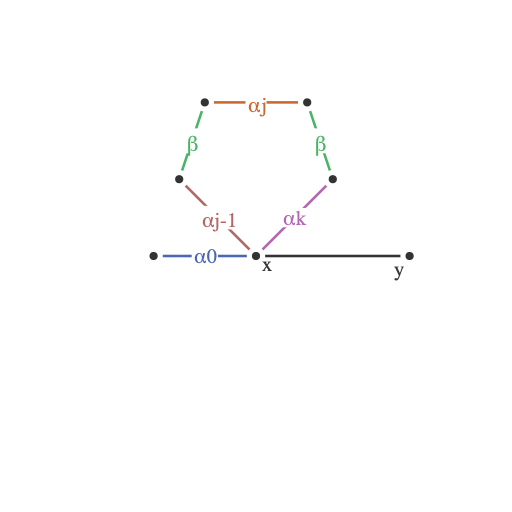
\includegraphics[scale=0.45]{chapters/dyskretna/colours/vizing/images/fan_case_three_before.png}
                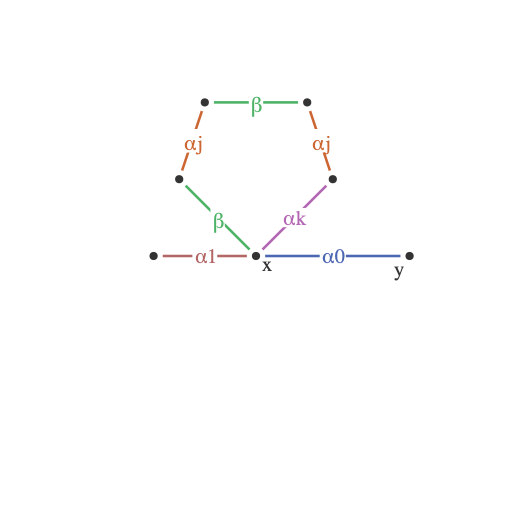
\includegraphics[scale=0.45]{chapters/dyskretna/colours/vizing/images/fan_case_three_after.png}
                \caption{Przekolorowanie gdy ścieżka z $x_k$ kończy się w $x_{j-1}$}
            \end{figure}
            
        \end{enumerate}
        
        
        
    \end{proof}

\section{Twierdzenie Brooksa}
\epigraph{
	Zgodnie z twierdzeniem Vizinga każdy graf można pokolorować przy użyciu co najwyżej $\Delta(G)+1$ kolorów. Twierdzenie Brooksa określa dla jakich grafów to ograniczenie jest osiągane.
}{\textit{
		Użytkownik ,,Esculapa'' na polskojęzycznej Wikipedii w artykule ,,Twierdzenie Brooksa''}}

Oczywiście przytoczona wypowiedź jest nonsensem gdyż, jak dobrze wiemy, twierdzenie Vizinga mówi o kolorowaniu \textbf{krawędziowym}.
Wypowiedzmy zatem poprawną formę twierdzenia Brooksa.

\begin{theorem}[Brooks]
	Jeśli spójny graf $G$ jest kliką lub cyklem nieparzystym to $\chi(G) = \Delta(G) + 1$.
	W przeciwnym razie $\chi(G) \leq \Delta(G)$
\end{theorem}

\begin{proof}
	Widzimy, że cykl nieparzysty wymaga użycia $3 = \Delta(G) + 1$ kolorów,
	a w przypadku kliki sąsiedzi każdego wierzchołka używają $\Delta(G)$ kolorów, a jeszcze jeden potrzebujemy na ten wierzchołek. Przyjmijmy zatem, że nasz graf $G$ nie jest
	ani cyklem nieparzystym ani kliką.

	Jeśli $\Delta(G) \leq 2$ to $G$ jest ścieżką lub cyklem parzystym i widzimy, że $G$ jest dwudzielny.

	Niech $\Delta(G) \geq 3$.

	Idea dowodu jest taka, że będziemy chcieli jakoś skonstruować kolorowanie używające co najwyżej $\Delta(G)$ kolorów. W związku z tym będziemy inkrementalnie odfiltrowywać grafy, dla których takie kolorowanie stworzymy.
	Przedstawiam zatem kolejne własności grafu, dla którego będzie się trzeba trochę bardziej namęczyć.

	\begin{enumerate}
		\item $G$ jest $\Delta$-regularny
		      Pokażemy, że w przeciwnym razie $col(G) \leq \Delta$
		      Jeśli $G$ nie jest $\Delta$-regularny to w $G$ istnieje wierzchołek $v$ o stopniu mniejszym niż $\Delta$.
		      Postawmy ten wierzchołek na końcu permutacji i spójrzmy na graf $G - v$.
		      $v$ miał jakichś sąsiadów, których stopień wynosił co najwyżej $\Delta$.
		      W takim razie po usunięciu $v$ jego byli sąsiedzi na pewno mają teraz stopień mniejszy niż $\Delta$
		      i możemy powtórzyć całe to rozumowanie aż skończą nam się wierzchołki i wygenerujemy całą permutację.
		      Zauważamy, że dzięki konstrukcji każdy wierzchołek ma na lewo mniej niż $\Delta$ sąsiadów i dostajemy $col(G) \leq \Delta$

		      Wybierzmy dowolny wierzchołek $v$ i oznaczmy $H = G - v$.
		      Sąsiadom $v$ zmniejszyliśmy stopień, zatem z powyższego wywodu wynika, że $H$ jest $\Delta$-kolorowalny.
		      Pokolorujmy zatem $H$ i przejdźmy do kolejnej własności.

		\item Sąsiedzi $v$ dostają parami różne kolory w kolorowaniu grafu $H$
		      W przeciwnym razie któryś z $\Delta$ kolorów jest wolny w $v$ i możemy go użyć kończąc kolorowanie.

		      Nazwijmy sąsiadów $v$ przez $v_1, ..., v_\Delta$ i niech będą pokolorowani kolorami $1, ..., \Delta$.

		      Oznaczmy $C_{ij} = H[\{v \in V \mid c(v) \in \{i, j\}]$ - podgraf indukowany
		      grafu $H$, który zawiera wszystkie wierzchołki w kolorach $i, j$

		\item Sąsiedzi $v_i, v_j$ leżą w tym samym komponencie grafu $C_{ij}$
		      W przeciwnym razie możemy wziąć komponent do którego należy $v_i$
		      i przekolorować go tak, że wierzchołki o kolorze $i$ dostają kolor $j$,
		      a te o kolorze $j$ dostają kolor $i$. Tym samym wierzchołki $v_i, v_j$
		      otrzymują oba kolor $j$ sprowadzając problem do poprzedniego podpunktu.

		\item Każdy $C_{ij}$ jest ścieżką.
		      Założmy że tak nie jest i weźmy pierwszy licząc od $v_i$ wierzchołek, który ma co najmniej trzech sąsiadów w $C_{ij}$ i nazwijmy go $x$.
		      Bez straty ogólności powiedzmy, że $x$ ma kolor $i$.
		      Rozważmy kolory jakie mają sąsiedzi $x$.
		      Co najmniej trzech sąsiadów ma kolor $j$, a pozostałych jest $\Delta - 3$
		      W takim razie sąsiedzi $x$ używają co najwyżej $\Delta - 2$ różnych kolorów. Oczywiście jeden z wolnych kolorów to $i$, ale możemy teraz przekolorować $x$ na ten drugi.
		      Ponieważ $x$ był pierwszym rozgałęzieniem między $v_i$ a $v_j$
		      to po przekolorowaniu $v_i$ oraz $v_j$ muszą leżeć w różnych komponentach nowego $C_{ij}$

		      \begin{figure}[ht]
			      \centering
			      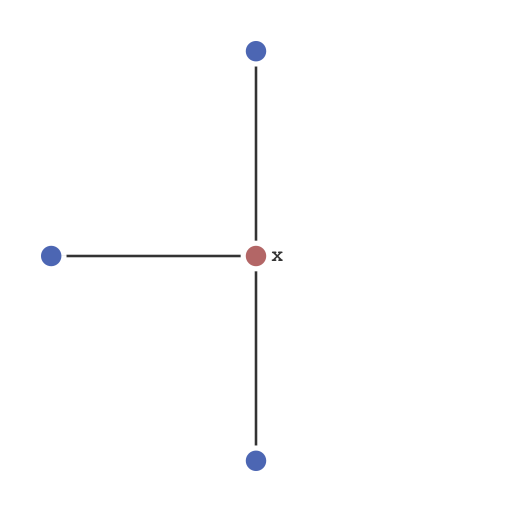
\includegraphics[scale=0.5]{images/brooks/branching_path.png}
			      \caption{Wierzchołek $x$ ma trzech sąsiadów w kolorze $j$}
		      \end{figure}

		\item Każde dwa $C_{ij}, C_{ik}, k \neq j$ przecinają się tylko w $v_i$
		      W przeciwnym razie istnieje wierzchołek $x$ w kolorze $i$,
		      który ma dwóch sąsiadów w kolorze $j$ i dwóch sąsiadów w kolorze $k$.
		      Jak się dobrze policzy to tak jak poprzednio wyjdzie nam, że jakiś kolor jest wolny i możemy zrobić ten sam myk z przekolorowaniem.

		      \begin{figure}[ht]
			      \centering
			      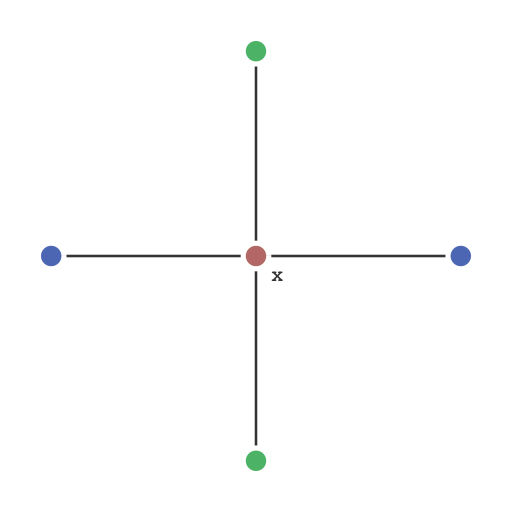
\includegraphics[scale=0.5]{images/brooks/branching_path_three_colors.png}
			      \caption{Wierzchołek $x$ ma dwóch sąsiadów w kolorze $j$ i dwóch w kolorze $k$}
		      \end{figure}

		\item Istnieje para $v_i, v_j$, która nie jest połączoną krawędzią.
		      W przeciwnym razie wierzchołki $v, v_1, ..., v_\Delta$ tworzą klikę, co jest sprzeczne z założeniem.

		      Bez straty ogólności powiedzmy, że $v_1$ i $v_2$ nie są połączone krawędzią. Jednak z własności (5) musi istnieć ścieżka między nimi. Niech więc $u$ to będzie pierwszy wierzchołek w kolorze $1$ na ścieżce od $v_2$ do $v_1$.

		      Teraz dzieje się magia.
		      W $C_{23}$ zamieniamy kolory $2$ i $3$ i takie kolorowanie przepuszczamy przez warunki $(2) - (5)$.
		      Jeśli w którymś miejscu udało nam się stworzyć dobre kolorowanie to super, a jeśli nie to ups.
		      Na szczęście zauważamy teraz fajną rzecz. Otóż wierzchołek $u$ nadal jest połączony ścieżką w kolorach $1$ i $2$ z wierzchołkiem $v_1$, zatem należy do komponentu $C_{12}$, ale z drugiej strony jest połączony krawędzią z wierzchołkiem $v_2$, który ma teraz kolor $3$ zatem należy też do komponentu $C_{13}$.
		      W takim razie nowe kolorowanie narusza warunek $(5)$ co już umiemy rozwiązać.

		      \begin{figure}[H]
			      \centering
			      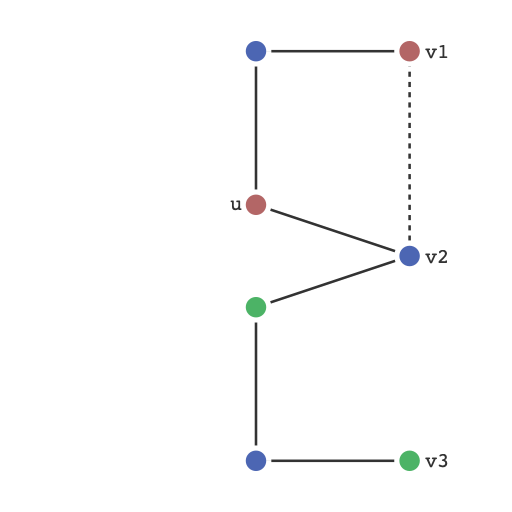
\includegraphics[scale=0.4]{images/brooks/disconnected_before_swap.png}
			      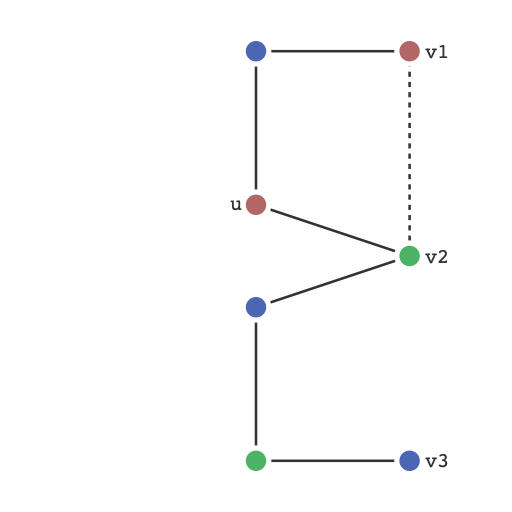
\includegraphics[scale=0.4]{images/brooks/disconnected_after_swap.png}
			      \caption{Wierzchołki $v_1$ i $v_2$ przed i po przekolorowaniu komponentu $C_{23}$}
		      \end{figure}


	\end{enumerate}

	To tyle, nie ma więcej warunków, które musimy rozważać. Fajnie.

\end{proof}

\section{Grafy bez trójkątów o dużej liczbie chromatycznej}
\subsection{Czemu interesują nas takie konstrukcje?}
\epigraph{A~komu to potrzebne? A~dlaczego?}{\textit{Pani z~Internetu, zapytana, czy należy w~Polsce zalegizować marihunaen}}
Mogłoby się wydawać, że liczba chromatyczna jest w jakiś sposób własnością lokalną grafu. To znaczy, oczywiście widzimy, że jeśli graf ma liczbę klikową \(\omega\), to musimy użyć przynajmniej \(\omega\) kolorów do jego pokolorowania. No dobra, ale może gdybyśmy lokalnie pokolorowali podgrafy będące dużymi klikami, to pozostałe części grafu już damy radę załatwić jakąś rozsądną liczbą dodatkowych kolorów? Prawda? Nieprawda. Okazuje się, że istnieją grafy, które nie zawierają nawet trójkątów, czyli mają \(\omega < 3\), ale mają też dowolnie dużą liczbę chromatyczną. Czyli niestety życie (przynajmniej jeśli dla kogoś życie opiera się na optymalnym kolorowaniu grafów) nie jest takie proste\dots
\subsection{Co będziemy konstruować?}
Pokażemy trzy sposoby zrobienia ciągu grafów \(G_3, G_4, \ldots\) (zaczynamy od \(3\)~bo dla \(0\), \(1\) i~\(2\) nie dzieje się nic ciekawego) takiego, że dla dowolnego \(n \geq 3\) będą zachodzić dwie własności:
\begin{itemize}
	\item \(\omega\pars{G_n} = 2\)
	\item \(\chi\pars{G_n} \geq n\)
\end{itemize}
Warto zwrócić uwagę, że \(n\)~\emph{nie będzie} liczbą wierzchołków w~takim grafie. Pamiętajmy --- ten ciąg grafów indeksujemy \emph{liczbą chromatyczną}, która nas interesuje, nie liczbą wierzchołków. Liczba wierzchołków wyjdzie w~praniu i~będzie zupełnie inna.

W każdym z~trzech sposobów zaczniemy od położenia \(G_3 = C_5\). Wszystko się zgadza --- \(C_5\) nie zawiera trójkąta i~ma \(\chi = 3\), bo jest cyklem nieparzystej długości. Resztę ciągu skonstruujemy rekurencyjnie.
\subsection{Konstrukcja Mycielskiego}
Załóżmy sobie, że mamy już \(G_n\), które spełnia wszystkie własności, jakie chcieliśmy. Chcemy teraz zrobić \(G_{n + 1}\). W~tym celu najpierw weźmiemy wierzchołki z~\(G_n\) --- nazwijmy je \(v_1, v_2, \ldots, v_N\), gdzie \(N = \left|V\pars{G_n}\right|\) (pamiętajmy tylko, że \(N \neq n\)). Doróbmy sobie jeszcze ,,kopie'' tych wierzchołków, tzn. odpowiadające im nowe wierzchołki, które nazwiemy \(v_1', v_2', v_N'\), i~dorzućmy jeszcze specjalny wierzchołek \(v^\ast\). Czyli, podsumowując, kładziemy
\begin{equation*}
	V\pars{G_{n + 1}} \coloneqq \left\{v_1, v_2, \ldots, v_N\right\} \cup \left\{v_1', v_2', \ldots, v_N'\right\} \cup \left\{v^\ast\right\}
\end{equation*}
A~jak będzie z~krawędziami? Po pierwsze, krawędzie między oryginalnymi wierzchołkami grafu \(G_n\) zostają jak były. Po drugie, każdy wierzchołek będący kopią łączymy z~wierzchołkiem specjalnym. Po trzecie, \emph{nie łączymy} żadnych dwóch kopii. I~po czwarte, każdą kopię łączymy z~sąsiadami odpowiadającego jej oryginału (czyli zapewniamy, że kopia ma takie samo sąsiedztwo jak oryginał, poszerzone jedynie o \(v^\ast\)). Formalnie:
\begin{equation*}
	E\pars{G_{n + 1}} \coloneqq E\pars{G_n} \cup \left\{v_iv^\ast : i \in [N]\right\} \cup \left\{v_i'v_j : i, j \in [N] \land v_iv_j \in E\pars{G_n} \right\}
\end{equation*}
Wyglądać to będzie mniej więcej tak:

\begin{figure}[H]
	\centering
	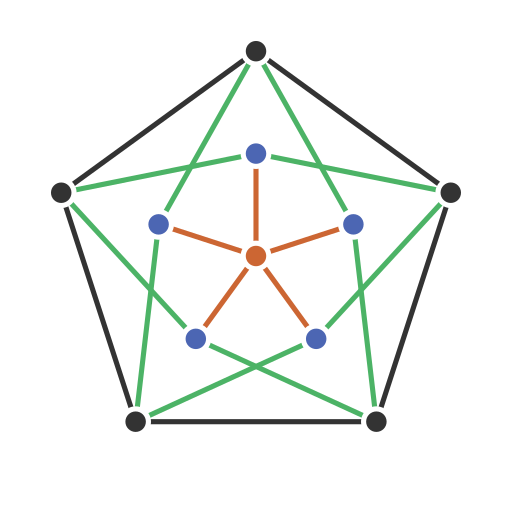
\includegraphics[scale=0.5]{images/mycielski_graph.png}
	\caption{Graf \(G_4\) w konstrukcji Mycielskiego}
\end{figure}

Przekonajmy się teraz, że stworzony \(G_{n + 1}\) posiada dwie cechy, których oczekiwaliśmy:
\begin{itemize}
	\item \(\omega\pars{G_{n + 1}} = 2\), czyli nie ma trójkątów. Zastanówmy się:
	      \begin{itemize}
		      \item na pewno \(v^\ast\) nie jest w~żadnym trójkącie, bo jego sąsiadami są tylko kopie, a~żadne dwie kopie nie są połączone
		      \item z~tego samego powodu żaden potencjalny trójkąt nie zawiera dwóch wierzchołków będących kopiami
		      \item trójkąt nie może składać się z~samych oryginałów, bo założyliśmy, że w~oryginalnym \(G_n\) nie było trójkątów
	      \end{itemize}
	      Zatem gdyby istniał trójkąt, to byłby on w~postaci \(v_iv_j'v_k\), dla pewnych \(i, j, k \in [N]\). Wtedy mielibyśmy oczywiście \(v_iv_k \in E\pars{G_{n + 1}}\), \(v_j'v_i \in E\pars{G_{n + 1}}\) oraz \(v_j'v_k \in E\pars{G_{n + 1}}\).\\
	      Ale pamiętajmy, że graf \(G_{n + 1}\) skonstruowaliśmy tak, żeby oryginalny wierzchołek i~jego kopia miały to samo sąsiedztwo (nie licząc \(v^\ast\)). Zatem skoro \(v_j'v_i \in E\pars{G_{n + 1}}\) oraz \(v_j'v_k \in E\pars{G_{n + 1}}\), to zachodzi \(v_jv_i \in E\pars{G_n}\) oraz \(v_jv_k \in E\pars{G_n}\). Krawędzi między oryginałami nie ruszaliśmy, więc skoro \(v_iv_k \in E\pars{G_{n + 1}}\) to również \(v_iv_k \in E\pars{G_n}\).\\
	      Ale z~tego wszystkiego wychodzi, że w~oryginalnym \(G_n\) istniał już trójkąt \(v_iv_jv_k\), a~przecież założyliśmy, że tak nie jest. Uzyskana sprzeczność dowodzi, że w~\(G_{n + 1}\) nie ma trójkątów.
	      \qed
	\item \(\chi\pars{G_{n + 1}} \geq n + 1\).
	      Załóżmy, że tak nie jest, tzn. \(\chi\pars{G_{n + 1}} \leq n\). Weźmy zatem kolorowanie \(c\), które o~tym świadczy i~poprawnie koloruje \(G_{n + 1}\) używając nie więcej niż \(n\)~kolorów. Przyjrzyjmy się teraz wierzchołkom-kopiom: widzimy na nich maksymalnie \(n - 1\) kolorów. Dlaczego? Gdyby zużywały one \(n\) kolorów, to zabrakłoby wolnego koloru na \(v^\ast\), który przecież jest połączony ze wszystkimi kopiami.\\
	      Świetnie, to teraz stwórzmy sobie kolorowanie \(c'\) grafu \(G_n\), które dla każdego \(i \in [N]\) będzie działać bardzo prosto:
	      \begin{equation*}
		      c'\pars{v_i} = \begin{cases}
			      c\pars{v_i}  & \iff c\pars{v_i} \neq c\pars{v^\ast} \\
			      c\pars{v_i'} & \iff c\pars{v_i} = c\pars{v^\ast}
		      \end{cases}
	      \end{equation*}
	      Innymi słowy: jeśli dany wierzchołek miał w~kolorowaniu \(c\)~taki kolor, jak specjalny wierzchołek \(v^\ast\), to dajemy mu kolor jego kopii, a~w~przeciwnym przypadku zostawiamy taki kolor, jaki był. Zauważmy, że \(c'\) jest poprawnym kolorowaniem \(G_n\). Dlaczego? Gdyby nie było, to znaczyłoby, że istnieje krawędź \(v_iv_j\) taka, że \(c'\pars{v_i} = c'\pars{v_j}\). Są trzy potencjalne wyjaśnienia tej sytuacji:
	      \begin{itemize}
		      \item w~kolorowaniu \(c\)~wierzchołki \(v_i\) i~\(v_j\) już miały ten sam kolor i~pozostał on niezmieniony --- ale to jest niemożliwe, bo kolorowanie \(c\)~było poprawne
		      \item w~kolorowaniu \(c\)~wierzchołki \(v_i\) i~\(v_j\) miały ten sam kolor \(c\pars{v^\ast}\), i~dla obydwu uległ on zmianie na ten sam kolor --- niemożliwe, jak wyżej
		      \item w~kolorowaniu \(c\)~wierzchołki wierzchołki miały różne kolory, przy czym dokładnie jeden z~nich miał kolor \(c\pars{v^\ast}\). Przyjmijmy bez straty ogólności, że był to \(v_i\). Skoro zatem \(c'\pars{v_i} = c'\pars{v_j}\), a~\(c\pars{v_i} = c\pars{v^\ast}\), to mamy \(c\pars{v_i'} = c'\pars{v_j} = c\pars{v_j}\). Ale to jest niemożliwe, bo skoro jest krawędź \(v_iv_j\), to jest też krawędź \(v_i'v_j\), a~w~poprawnym kolorowaniu \(c\)~nie mogło być dwóch sąsiednich wierzchołków w~tym samym kolorze.
	      \end{itemize}
	      Uzyskane sprzeczności dowodzą, że \(c'\)~rzeczywiście jest poprawnym kolorowaniem \(G_n\) przerobionym z~kolorowania \(c\), które używało nie więcej, niż \(n\)~kolorów. Ale zauważmy, że w~\(c'\)~pozbyliśmy się  jednego z~kolorów, mianowicie \(c\pars{v^\ast}\). Zatem \(c'\)~jest poprawnym \(\pars{n - 1}\)-kolorowaniem grafu \(G_n\), co jednak jest niemożliwe, bo przecież założyliśmy, że \(\chi\pars{G_n} \geq n\). Uzyskana sprzeczność dowodzi ostatecznie, że istotnie \(\chi\pars{G_{n + 1}} \geq n + 1\).
	      \qed
\end{itemize}
\subsection{Konstrukcja Tutte'a}
Ponownie zakładamy, że mamy działające \(G_n\) i~chcemy zrobić \(G_{n + 1}\). Przyjmijmy \(N = \left|V\pars{G_n}\right|\). Ta konstrukcja jest bardzo prosta: najpierw tworzymy sobie \(n \cdot \pars{N - 1} + 1\) zupełnie nowych wierzchołków --- nazwijmy je \emph{wierzchołkami głównymi}. Teraz przy każdym \(N\)-elementowym podzbiorze tych wierzchołków tworzymy kopię \(G_n\) i~łączymy wierzchołki główne z~odpowiadającymi im wierzchołkami z~kopii \(G_n\) (w~dowolnym porządku, byle każdy wierzchołek główny z~podzbioru miał dokładnie jednego kolegę w~odpowiadającej temu podzbiorowi kopii). Najłatwiej to zobaczyć na poniższym rysunku:

\begin{figure}[H]
	\centering
	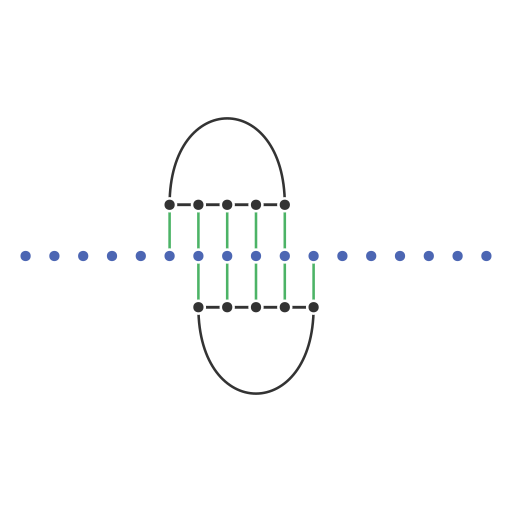
\includegraphics[scale=0.5]{images/tutte_graph.png}
	\caption{Fragment \(G_4\) w konstrukcji Tutte'a}
\end{figure}

Między poszczególnymi kopiami \(G_n\) nie dajemy żadnych krawędzi. Podobnie nie dajemy żadnych krawędzi między wierzchołkami głównymi. I~gotowe --- mamy nasze \(G_{n + 1}\)! Przyjrzyjmy się, czemu taki graf spełnia nasze wymagania:
\begin{itemize}
	\item brak trójkątów --- oczywiście żadnego trójkąta nie ma:
	      \begin{itemize}
		      \item w~żadnej kopii \(G_n\), bo założyliśmy, że \(G_n\) jest bez trójkątów
		      \item pomiędzy kopiami \(G_n\), bo powiedzieliśmy, że różnych kopii w~żaden sposób nie łączymy
		      \item wśród wierzchołków głównych, bo między nimi nie ma krawędzi
	      \end{itemize}
	      Zatem jedyny możliwy trójkąt musiałby mieć jeden wierzchołek główny i~dwa wierzchołki z~kopii. Ale te dwa z~kopii nie mogą być w~jednej kopii \(G_n\), bo każdy wierzchołek główny ma dokładnie jednego kolegę w~każdej kopii. Nie mogą też być w~różnych kopiach \(G_n\), bo aby domknąć trójkąt, musiałyby się łączyć, a~między kopiami nie ma krawędzi. Zatem w~\(G_{n + 1}\) nie istnieją trójkąty.
	      \qed
	\item \(\chi\pars{G_{n + 1}} \geq n + 1\). Załóżmy, że tak nie jest, czyli \(\chi\pars{G_{n + 1}} \leq n\). Weźmy zatem kolorowanie, które o~tym świadczy. Ponieważ jest \(n \cdot \pars{N - 1} + 1\) głównych wierzchołków, to z~zasady szufladkowej musi istnieć tam \(N\)~wierzchołków, które mają taki sam kolor, powiedzmy \(k\). Rozważmy teraz kopię skonstruowaną przy tym \(N\)-elementowym podzbiorze wierzchołków głównych. Żaden z~wierzchołków w~tej kopii nie może mieć koloru \(k\), ponieważ jest połączony z~odpowiadającym mu wierzchołkiem głównym. A~to oznacza, że ta kopia \(G_n\) została pokolorowana nie więcej niż \(n - 1\) kolorami. Ale to jest przecież niemożliwe, bo założyliśmy, że \(\chi\pars{G_n} \geq n\). Uzyskana sprzeczność pokazuje, że istotnie \(\chi\pars{G_{n + 1}} \geq n + 1\).
	      \qed
\end{itemize}

\subsection{Konstrukcja Zykova}
Również zakładamy, że mamy działające \(G_n\). Będziemy tworzyć \(G_{n + 1}\). Na dobry początek zróbmy sobie \(n\)~rozłącznych kopii grafu \(G_n\). Teraz dla każdego możliwego wyboru, wyróżniającego po jednym wierzchołku z~każdej kopii, dodajemy jeden wierzchołek ,,na dole'' i~łączymy go z~tymi wyróżnionymi. Żadnych innych krawędzi nie dodajemy. Ponownie, najlepiej to zobaczyć na rysunku:

\begin{figure}[H]
	\centering
	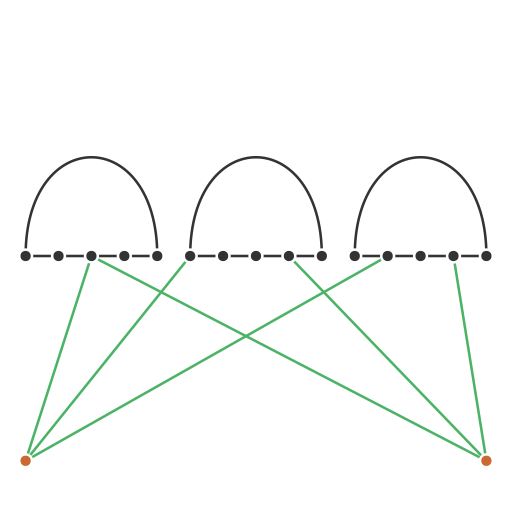
\includegraphics[scale=0.5]{images/zykov_graph.png}
	\caption{Fragment \(G_4\) w konstrukcji Zykova}
\end{figure}

To będzie nasze \(G_{n + 1}\). Zbadajmy, czemu to działa:
\begin{itemize}
	\item brak trójkątów --- na pewno trójkąt nie znajdzie się:
	      \begin{itemize}
		      \item w~żadnej kopii \(G_n\), bo z~założenia nie ma tam trójkątów
		      \item pomiędzy różnymi kopiami \(G_n\), bo nie są one wcale połączone
		      \item wśród wierzchołków ,,na dole'', bo nie ma między nimi żadnych krawędzi
	      \end{itemize}
	      Zatem jedyny potencjalny trójkąt musiałby mieć jeden wierzchołek na dole i~dwa w~kopiach \(G_n\). Te dwa ,,górne'' nie mogą być jednak w~tej samej kopii \(G_n\), bo każdy wierzchołek z~dołu w~danej kopii ma \emph{dokładnie jednego} sąsiada. Nie mogą też być w~różnych kopiach \(G_n\), bo musiałyby być połączone, a~przecież kopie się nie łączą. Czyli żaden trójkąt nie może się pojawić w~\(G_{n + 1}\).
	      \qed
	\item \(\chi\pars{G_{n + 1}} \geq n + 1\). Pokażemy, że nie da się pokolorować \(G_{n + 1}\) używając \(n\)-kolorów. Załóżmy do dowodu nie wprost, że jest to możliwe, i~weźmy takie poprawne \(n\)-kolorowanie. Powiedzmy, że te kolory to \(1, 2, \ldots, n\). Oczywiście każda kopia \(G_n\) używa wszystkich \(n\)~kolorów, bo \(\chi\pars{G_n} \geq n\). Zatem z~pierwszej kopii wybierzmy dowolny wierzchołek w~kolorze \(1\), z~drugiej kopii dowolny wierzchołek w~kolorze \(2\), \dots, z~\(n\)-tej kopii wierzchołek w~kolorze \(n\). To jest wybór po jednym wierzchołku z~każdej kopii, więc na dole jest wierzchołek połączony z~nimi wszystkimi. Ups\dots Ale to oznacza, że zabraknie na niego wolnego koloru, bo dla każdego z~dostępnych \(n\)~kolorów ten ,,dolny'' wierzchołek jest połączony z~wierzchołkiem w~tym kolorze ,,na górze''. Uzyskana sprzeczność dowodzi nierówności \(\chi\pars{G_{n + 1}} \geq n + 1\).
	      \qed
\end{itemize}


\section{Shift grafy}
Shift grafy są kolejnym przykładem rodziny grafów bez trójkątów ale o~dowolnie dużej liczbie chromatycznej. Czemu są jako osobne wymaganie egzaminacyjne? Cytując Tadeusza Sznuka, odpowiedź brzmi: nie wiem, choć się domyślam. Otóż konstrukcja shift grafów (znana też jako konstrukcja Erdősa–Hajnala) jest jawna, natomiast te poprzednie są rekurencyjne. Konkretniej: będziemy konstruować ciąg takich grafów $G_n = \pars{V_n, E_n}$, że $\omega\pars{G_n} = 2$ oraz $\chi\pars{G_n} \geq \left\lceil\log_2n\right\rceil$. Zrobimy to następująco:
\begin{gather*}
	V_n = \left\{[i, j] : 1 \leq i < j \leq n\right\}\\
	\{[i, j], [k, l]\} \in E_n \iff j = k
\end{gather*}
Innymi słowy, wierzchołkami naszego grafu będą przedziały o~końcach ze~zbioru $[n]$, bez przedziałów będących pojedynczym punktem, natomiast dwa przedziały są połączone krawędzią wtedy, gdy koniec jednego dotyka początku drugiego. Nie ma tutaj trójkątów. Dlaczego? Trójkąt musiałby być w postaci $[i, j], [j, k], [k, i]$, a~taka trójka przedziałów oczywiście nie może istnieć na prostej, bo wynikałoby z~tego coś w~stylu $i < j < k < i$.

Przyszedł czas udowodnić fakt o~liczbie chromatycznej. Weźmy dowolne $k$-kolorowanie $G_n$ i~nazwijmy je $c$. Pokażemy, że $2^k \geq n$, czyli $k \geq \log_2n$, a~ponieważ pracujemy na liczbach całkowitych, to dostaniemy z~tego $k \geq \left\lceil\log_2n\right\rceil$. Zdefiniujmy zbiory $C_1, C_2, \ldots, C_n$ następująco:
\begin{equation*}
	C_i = \left\{b \in [k] : b = c\pars{[j, i]} \text{ dla } j < i\right\}
\end{equation*}
Mówiąc najprościej, w~zbiorze $C_i$ są kolory przedziałów kończących się na punkcie $i$. Teraz pokażemy, że $C_i \neq C_j$ dla $i \neq j$. W~tym celu pokażemy, że dla każdej pary $j > i$ istnieje kolor należący do $C_j$ i~nienależący do $C_i$, czyli świadczący o~różności tych zbiorów. Jak tego dokonamy? Okazuje się, że bardzo prosto. Weźmy przedział $[i, j]$. Ma on jakiś kolor $b \in [k]$. Żaden przedział kończący się na $i$~nie może mieć koloru $b$, bo ma krawędź do $[i, j]$. Zatem $b \not\in C_i$. Ale oczywiście przedział $[i, j]$ kończy się na\dots $j$, a~skoro ma kolor $b$, to $b \in C_j$.

Czyli, podsumowując, mamy zbiory $C_1, C_2, \ldots, C_n$ i~wszystkie różne. Oczywiście wszystkie są też podzbiorami $[k]$. Z~zasady szufladkowej wynika, że w~takim razie $n \leq 2^k$, co kończy dowód.
\qed

\section{Grafy przecięć kwadratów}
\begin{theorem}
	Liczba kolorująca w grafach przecięć kwadratów na płaszczyźnie ograniczona jest przez $4 \omega - 3$.
\end{theorem}
\begin{proof}
	Ustalmy sobie porządek na kwadratach taki, że jeśli dany kwadrat $x$ ma krótszy bok niż kwadrat $y$, to $y$ jest w permutacji przed $x$. Jeżeli ktoś nie wie jak działają permutacje wierzchołków dla liczby kolorującej to sugeruję poczytać najpierw jak to wszystko działa. W sumie to nie sugeruję tylko nakazuję.

	Wracając, jako że im mniejszy jest kwadrat tym później jest w permutacji wierzchołków do cola, wszystkie kwadraty które są ,,na lewo'' od niego i mają do niego krawędź (tj. przecinają się z nim) muszą ,,w sobie'' mieć któryś z 4 wierzchołków tego kwadratu (przypominam że w grafie przecięć kwadratów na płaszczyźnie z definicji wszystkie kwadraty mają 2 krawędzie pionowo i 2 poziomo, nie dopuszczamy jakiegoś obracania). Fakt ten wynika z dowodu \textit{to widać}, ale serio -- jeśli ktoś znalazł sposób na władowanie kwadratu o większym boku w taki o mniejszym boku w grafie przecięć kwadratów \textbf{bez obracania} w taki sposób, że kwadrat o mniejszym boku nie ma żadnego wierzchołka w tym o większym boku, sugeruję kontakt z psychologiem.

	No i fajnie, bo teraz ograniczam sobie liczbę kwadratów które mam ,,na lewo'' przez $4\omega - 4$. Dlaczego? Bo wszystkie kwadraty które przecinają wierzchołek $x$ mojego kwadratu (przypominam że kwadrat ma 4 wierzchołki, to zaraz będzie ważne) muszą formować jakąś klikę (no w sensie wszystkie mają punkt wspólny w postaci tego wierzchołka). Obecny kwadrat też wpada do tej kliki, więc wychodzi mi maksymalnie $\omega - 1$ sąsiadów na każdy wierzchołek. I w sumie to tyle, mamy ograniczenie liczby kolorującej więc mamy ograniczenie liczby chromatycznej. Fajnie.
\end{proof}



\section{Grafy przecięć prostokątów}
\subsection{Liczba kolorująca}
Czy jesteśmy w stanie ograniczyć liczbę kolorującą przez funkcję od liczby klikowej w grafie przecięć prostokątów na płaszczyźnie?
\begin{theorem}
	Nie.
\end{theorem}
\begin{proof}
	Możemy stworzyć klikę $K_{n,n}$ w tej klasie grafów. No i w sumie tyle.
	\begin{figure}[H]
		\centering
		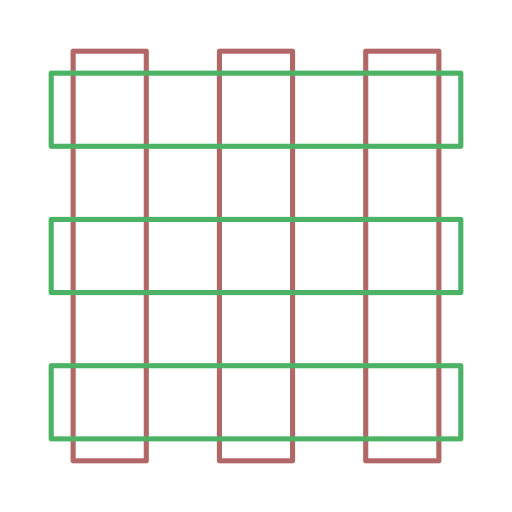
\includegraphics[scale=0.35]{images/objects_on_plane/k_3_3_of_rectangles.png}
		\caption{$K_{3,3}$ jako przecięcia prostokątów}
	\end{figure}
\end{proof}
\subsection{Liczba chromatyczna}

Nie potrafimy ograniczyć liczby kolorującej to może chociaż chromatyczną umiemy? Okazuje się, że tak.
\begin{theorem}
	Liczba chromatyczna w grafach przecięć prostokątów na płaszczyźnie ograniczona jest przez $\omega \cdot (8\omega - 7)$.
\end{theorem}
\begin{proof}
	Kolorujemy prostokąty na płaszczyźnie w dość zabawny sposób, bo każdy kolor będzie składał się z pary liczb.
	Pierwsza współrzędna będzie przyjmowała wartości od $1$ do $\omega$, natomiast druga od $1$ do $8\omega - 7$.
	Intuicyjnie będzie odpowiadało to podzieleniu prostokątów na $\omega$ warstw, z których każdą z osobna będziemy umieli pokolorować na $8\omega - 7$ kolorów.

	Zacznijmy od pierwszej współrzędnej.
	Powiemy, że dwa prostokąty \textbf{krzyżują się} jeśli przecinają się, ale wnętrze (bez brzegu) jednego nie zawiera wierzchołków drugiego.
	Jeżeli skierujemy relację krzyżowania w ten sposób, że
	$u \leq v$ gdy $u$ jest węższy niż $v$ to okazuje się, że dostaniemy częściowy porządek.
	Możemy zauważyć, że łańcuch w tym porządku to ciąg coraz węższych i dłuższych prostokątów o wspólnym ,,środku'', więc tworzą one klikę o maksymalnym rozmiarze $\omega$.

	\begin{figure}[H]
		\centering
		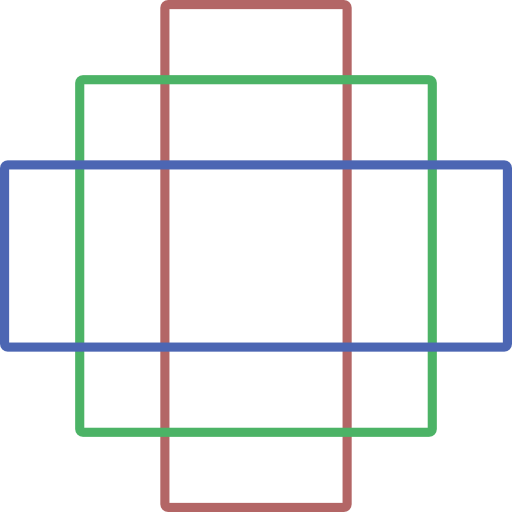
\includegraphics[scale=0.75]{images/objects_on_plane/rectangle_clique.png}
		\caption{,,Krzyżujące się'' prostokąty tworzące klikę; każdy prostokąt dostaje inny kolor na pierwszej współrzędnej}
	\end{figure}


	Skoro rozmiar najdłuższego łańcucha to $\omega$ to możemy skorzystać z twierdzenia dualnego do Dilwortha i podzielić prostokąty na $\omega$ antyłańcuchów $A_1, ..., A_\omega$,
	które intuicyjnie będą odpowiadały grupom prostokątów, które się nie krzyżują parami.
	Następnie na pierwszej współrzędnej każdy prostokąt dostaje numer antyłańcucha do którego trafił.

	Okazuje się, że dla prostokątów mających ten sam pierwszy kolor (a więc takich które się nie krzyżują) jesteśmy już w stanie ograniczyć liczbę kolorującą, a więc i liczbę chromatyczną. Robimy to w dosyć sprytny sposób.  Mianowicie zauważamy, że skoro prostokąty się nie krzyżują, gdy przecinają się one to musi być tak że jakiś wierzchołek jednego jest w drugim (lub vice versa).

	Co robimy z tym fascynującym faktem? Otóż majstrujemy sobie graf \textbf{skierowany} na prostokątach w taki sposób,
	że krawędź z prostokąta $u$ do prostokąta $v$ mamy, gdy $u$ ma wierzchołek wewnątrz $v$.
	\begin{figure}[H]
		\centering
		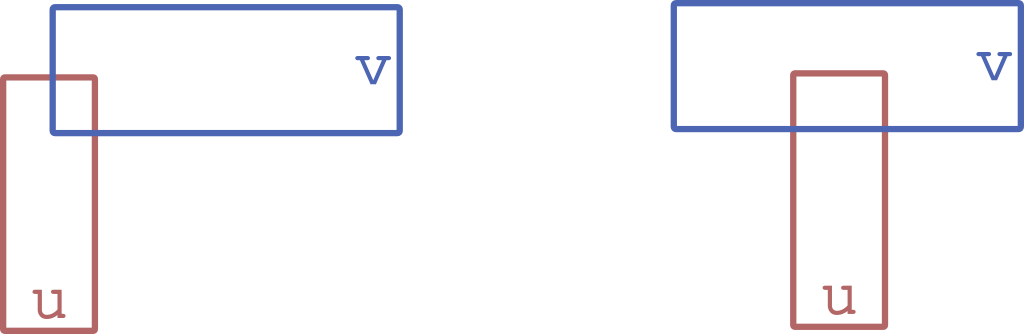
\includegraphics[scale=0.75]{images/objects_on_plane/rectangle_edges.png}

		\caption{po lewej mamy krawędzie $(u, v)$ oraz $(v, u)$, po prawej tylko $(u, v)$}
	\end{figure}

	Podobnie jak przy grafach przecięć kwadratów, zauważamy że z jednego prostokąta może wychodzić maksymalnie $4\omega - 4$ krawędzi (bo każdy wierzchołek może się zawierać w co najwyżej $\omega - 1$ prostokątów).
	W takim razie oszacowanie górne na liczbę krawędzi w grafie wynosi $|E| \leq |V| \cdot (4\omega - 4)$. Jednocześnie wiemy, że \begin{equation*}
		\sum_{v \in V} deg(v) = 2 \cdot |E|
	\end{equation*}
	Skąd
	\begin{equation*}
		\sum_{v \in V} deg(v) = 2 \cdot |E| \leq |V| \cdot (8 \omega - 8)
	\end{equation*}
	\begin{equation*}
		\frac{\sum_{v \in V} deg(v)}{|V|} \leq 8 \omega - 8
	\end{equation*}
	Należy zauważyć, że po lewej stronie mam średnią arytmetyczną stopni wszystkich wierzchołków w tym grafie. Ponieważ jest ona mniejsza lub równa $8 \omega - 8$, to wiem że istnieje na pewno wierzchołek który ma stopień mniejszy bądź równy $8\omega - 8$ (tak działa średnia arytmetyczna). To oczywiście tłumaczy się na to, że istnieje prostokąt o maksymalnym stopniu $8\omega - 8$ w grafie przecięć prostokątów. No a skoro tak, to prostokąt taki mogę sobie zawsze ,,wrzucić'' zawsze na koniec permutacji do liczby kolorującej, ,,odgryźć'' go od grafu i znowu wrzucić prostokąt o takim maksymalnym stopniu i tak dalej. Tym samym osiągnęliśmy ograniczenie na liczbę kolorującą w postaci $col(G) \leq 8\omega - 7$ (czyli również ograniczyliśmy liczbę możliwych kolorów ,,na drugiej współrzędnej'' w ten sposób).

	Podsumowując: skoro na pierwszej współrzędnej mamy $\omega$ możliwych wartości, a na drugiej $8\omega - 7$ to razem używamy $\omega \cdot (8\omega - 7)$ kolorów.

\end{proof}


\section{Grafy planarne}
\subsection{Wzór Eulera}
\begin{theorem}
	Przez $v$ oznaczmy liczbę wierzchołków, $e$ liczbę krawędzi a $f$ liczbę ścian spójnego grafu planarnego $G$. Mamy:
	\begin{equation}
		v - e + f = 2
	\end{equation}
\end{theorem}
\begin{proof}
	Robimy sobie drzewo rozpinające naszego grafu $G$ (ważne założenie, że jest on spójny). Drzewa to dosyć przyjemna klasa grafów, bo jeśli mają $n$ wierzchołków to mają $n-1$ krawędzi. Ponadto mają tylko jedną ścianę (zewnętrzną). Zatem $f = 1$, a $e = v-1$. W takim razie dla drzewa rozpinającego naszego grafu planarnego zachodzi teza. Teraz zauważamy, że jak dodamy jakąś krawędź to to nadal zostaje równe 2, bo $f$ zwiększa się o jeden i $e$ zwiększa się o jeden. Dokładając zatem krawędź po krawędzi otrzymujemy wyjściowy graf planarny, w którym zachodzi teza.
\end{proof}

\subsection{Liczba kolorująca}
Pokażemy, że w dowolnym grafie planarnym $G$ istnieje wierzchołek o stopniu równym co najwyżej 5. Wtedy w oczywisty sposób ograniczymy liczbę kolorującą od góry przez 6 (bo w takim razie $\delta(G) \leq 5$ dla dowolnego grafu planarnego, więc będziemy mogli zastosować fajny wzór na liczbę kolorującą). Jeśli nie wiesz o jaki wzór mi chodzi, rekomenduję cofnięcie się do rozdziału o liczbie kolorującej, gdzie ten jest dowodzony. Do udowodnienia zostaje zatem pokazanie, że w każdym grafie planarnym istnieje wierzchołek o stopniu co najwyżej 5.

\begin{theorem}
	W każdym grafie planarnym istnieje wierzchołek o stopniu co najwyżej 5.
\end{theorem}
\begin{proof}
	Załóżmy nie wprost, że tak nie jest. Ponadto zakładamy że graf jest spójny (bo jak nie jest, to prowadzimy rozumowanie dla grafu spójnego dla jakiegoś jego komponentu spójnego). Ze wzoru eulera mamy, że $v - e + f = 2$. Jednocześnie z założenia nie wprost mamy, że każdy wierzchołek ma stopień co najmniej 6. Stosujemy lemat o uściskach dłoni:
	\begin{equation*}
		\sum_{u \in V} deg(u) = 2 \cdot |E|
	\end{equation*}
	Korzystając z założenia nie wprost, że dla dowolnego $u$ jest tak, że $(deg(u) \geq 6)$:
	\begin{equation*}
		\sum_{u \in V} deg(u) = 2 \cdot |E| \geq 6 \cdot v
	\end{equation*}
	czyli $e \geq 3v $. Teraz wykonuję fikołek, bo mówię że mój graf ma co najmniej 3 wierzchołki. Jeśli ma mniej, to w sumie teza jest oczywista. Jeśli ma co najmniej 3 wierzchołki zaś, to mogę wykonać bardzo ciekawą obserwację: mianowicie każda ściana ,,wydzielana'' jest przez co najmniej 3 krawędzie. W dodatku każda krawędź ma ,,kontakt'' z maksymalnie dwiema ścianami.

	Teraz wykonuję bardzo śmieszną czynność, bowiem robię coś niezwykle poetyckiego, co wręcz prosi się o rysunek; na każdej ścianie ,,kładę'' 3 ,,monety''. Każda z tych monet idzie do różnych krawędzi. Jedna krawędź dostanie maksymalnie 2 monety, ale na każdej ścianie położono 3 monety. Stąd mam, że w grafie planarnym, który ma co najmniej 3 wierzchołki:
	\begin{equation*}
		2e \geq 3f
	\end{equation*}
	Jest to najbardziej machany dowód przez rysowanie który znam, ale jest on prezentowany również na wykładach. I okazuje się, że jak podstawimy tę własność do wzoru Eulera otrzymamy coś bardzo ciekawego. Mianowicie:
	\begin{equation*}
		v - e + f = 2
	\end{equation*}
	\begin{equation*}
		f = 2 - v + e
	\end{equation*}
	\begin{equation*}
		3f = 6 - 3v + 3e
	\end{equation*}
	\begin{equation*}
		6 - 3v + 3e = 3f \leq 2e
	\end{equation*}
	\begin{equation*}
		6 - 3v + 3e \leq 2e
	\end{equation*}
	\begin{equation*}
		6 - 3v + e \leq 0
	\end{equation*}
	\begin{equation*}
		e \leq 3v - 6
	\end{equation*}
	Zaraz chwilunia, ale z założenia nie wprost mieliśmy że $e \geq 3v$. Mielibyśmy wtedy, że $3v \leq 3v-6$ skąd $0 \leq -6$. Brzmi trochę jak sprzeczność.
\end{proof}

\subsection{5-kolorowalność}
\begin{theorem}[Ograniczenie górne na liczbę chromatyczną w grafach planarnych]
	W grafie planarnym $G$ zachodzi:
	\begin{equation}
		\chi(G) \leq 5
	\end{equation}
\end{theorem}


\begin{proof}
	Dowód przez indukcję. Zakładamy, że w każdym grafie planarnym jest tak, że istnieje wierzchołek o stopniu co najwyżej 5 (co zostało już udowodnione wcześniej).

	Przypadek bazowy indukcji (graf planarny stanowiący po prostu jeden wierzchołek) jest trywialny.

	Załóżmy teraz, że mam sobie graf planarny $G = (V,E)$. Biorę sobie wierzchołek $x$ taki, że ma stopień mniejszy lub równy 5. Z założenia indukcyjnego graf indukowany na wierzchołkach $V \setminus \{x\}$ można pokolorować 5 kolorami (lub mniej). Zakładam, że $x$ ma dokładnie 5 sąsiadów, bo jeśli ma ich mniej na pewno jest jakiś ,,wolny'' z 5 kolorów na które mogę go pokolorować i otrzymać poprawne kolorowanie. Sąsiadów $x$ oznaczam jako $v_1, v_2, v_3, v_4$ i $v_5$. Bez straty ogólności zakładamy, że w tej kolejności zgodnie z ruchem wskazówek zegara. Zakładam że sąsiad $v_i$ ma kolor $i$ (czyli że każdy sąsiad ma inny kolor; jeśli tak nie jest, to od razu mam poprawne kolorowanie, bo znowu biorę sobie ,,wolny'' kolor).

	Zauważam teraz fajną rzecz: między dowolnymi dwoma sąsiadami $v_i$ i $v_j$ musi istnieć ścieżka z wierzchołkami o kolorach $i, j, i, \dots, i, j$. Wynika to z faktu, że gdyby takiej ścieżki nie było, to mógłbym wziąć sobie $v_i$ i przekolorować go na kolor $j$. Jego sąsiada w kolorze $j$ (o ile taki by istniał) na kolor $i$ i tak dalej. Otrzymałbym poprawne kolorowanie, ale $x$ miałby dwóch sąsiadów w kolorze $j$ (jeśli $v_i$ i $v_j$ są połączone to taki zabieg nadal daje poprawne kolorowanie, ale $v_j$ dostaje kolor $i$ i w sumie to nic nie osiągnąłem) i mógłbym mu dać kolor $i$.

	Skoro tak, to między $v_1$ i $v_3$ istnieje taka ,,ścieżka dwukolorowa''. Zauważam jednak, że wtedy nie może istnieć taka ścieżka między $v_2$ i $v_4$ (znaczy zależy jak je rozrysujemy, ale jak zobaczycie rysunek to się wyjaśni o co mi chodzi -- pomysł jest taki, że $v_2$ jest poniekąd ,,odizolowany'' przez ścieżkę między $v_1$ a $v_3$). To oznacza, że zgodnie z opisaną powyżej procedurą mogę sobie po prostu przekolorować $v_2$ na kolor $4$, a wierzchołkowi $x$ dać kolor $2$, otrzymując poprawne kolorowanie. Nie mam pojęcia jak formaliści chcieliby to sformalizować, ale ci pewnie nadal siedzą nad definicją spaceru rozgałęziającego się w drzewie Steinera.

	\begin{figure}[H]
		\centering
		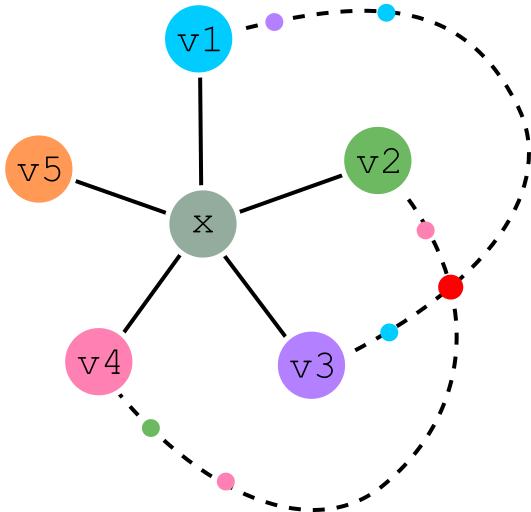
\includegraphics[scale=0.5]{images/graf_planarny.png}
		\caption{Niemożliwe jest połączenie ,,ścieżką dwukolorową'' wierzchołka $v_2$ z $v_4$, jeśli takową już połączyliśmy wierzchołek $v_1$ z wierzchołkiem $v_3$.}
	\end{figure}

\end{proof}

\subsection{5-wybieralność}
\epigraph{To było coś takiego?}{\textit{Student TCSu o 5-wybieralności, na chwilę przed wejściem na egzamin}}
Jeśli myślisz że skoro tego nie ma w wymaganiach więc nie będzie na egzaminie, to się grubo mylisz. Byli już tacy, którzy na tym się przejechali. Nie wiem z czego wynika brak tego tematu w wymaganiach, ale czuję się zobowiązany go opisać.

\subsubsection{Co to jest w ogóle 5-wybieralność?}
Podejrzewam, że spora część czytających zaczęła wyświetlać obrazek \textit{co.png} na twarzy gdy ujrzała frazę \textit{5-wybieralność}. Z tego względu pozwolę sobie zdefiniować, o co w ogóle tutaj chodzi.

Mówimy, że graf $G$ jest $k$-wybieralny, jeżeli po przydzieleniu każdemu wierzchołkowi jakiejś listy co najmniej $k$ różnych kolorów na które można go pokolorować, możliwe jest jego pokolorowanie (dla dowolnego takiego przydziału list).

\textit{Przykład.} Klika $K_3$ (znana wśród niektórych jako \textit{trójkąt}) jest 3-wybieralna. Klika dwudzielna $K_{3,3}$ nie jest natomiast $2$-wybieralna (mimo bycia $2$-kolorowalną).

\begin{figure}[H]
	\centering
	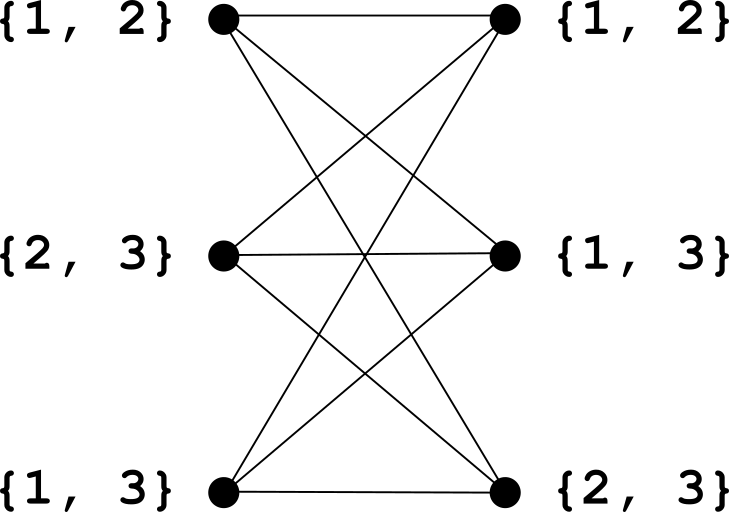
\includegraphics[scale=0.8]{images/K33.png}
	\caption{Klika dwudzielna $K_{3,3}$ z $2$-elementowymi listami takimi, że grafu nie da się pokolorować poprawnie.}
\end{figure}

Zauważmy również, że jeśli graf $G$ jest $k$-wybieralny, to $\chi(G) \leq k$; każdemu wierzchołkowi wystarczy dać listę $k$ kolorów od $1$ do $k$ (bo da się go pokolorować dla dowolnego przydziału list, w szczególności również i do takiego).

Najmniejsze takie $k$, że graf $G$ jest $k$-wybieralny, będziemy oznaczać jako $\chi_{_l}(G)$.

\subsubsection{5-wybieralność grafów planarnych}
Niech $G$ będzie grafem planarnym. Wtedy zachodzi:
\begin{theorem}[O 5-wybieralności grafów planarnych]{
		\begin{equation}
			\chi_{_l}(G) \leq 5
		\end{equation}
	}
\end{theorem}

\begin{proof}
	Dowód przeprowadzimy indukcją, do której będziemy potrzebowali nieco silniejszych założeń niż tylko, że $G$ jest planarny i wszystkie listy są pięcioelementowe.

	Założenia, które czynimy:
	\begin{enumerate}
		\item Każda wewnętrzna ściana jest trójkątem.
		\item Do ściany zewnętrznej przyległe są dwa sąsiadujące wierzchołki $u$ i $v$ takie, że
		      $$ |L(u)| = |L(v)| = 1, L(u) \neq L(v) $$
		\item Pozostałe wierzchołki przyległe do ściany zewnętrznej mają listy długości 3
		\item Wszystkie pozostałe wierzchołki grafu mają listy 5-elementowe
	\end{enumerate}

	Zauważmy, że dowolny graf planarny wraz z listami 5-elementowymi jesteśmy w stanie przekształcić w graf spełniający powyższe warunki (dodając krawędzie i skracając odpowiednio listy), a uzyskane kolorowanie będzie poprawne w wyjściowym grafie.

	Robimy indukcję po liczbie wierzchołków; Widzimy, ze gdy $G$ ma co najwyżej 3 wierzchołki to teza w trywialny sposób zachodzi.

	Rozpatrzmy teraz graf $G$ z jakimiś wierzchołkami $v, u$ które są na ścianie zewnętrznej. Rozważmy sąsiada $v$ ze ściany zewnętrznej (innego niż $u$). Nazwiemy go $w$. Rozpatrujemy teraz 2 przypadki:

	Gdy z $w$ wychodzi jakaś ,,cięciwa'', tj. krawędź łącząca się z innym wierzchołkiem na ścianie zewnętrznej różnym od dwóch, z którymi $w$ łączy się ,,normalnie''. Wtedy otrzymuję ,,podział'' grafu planarnego na 2 podgrafy. Z założenia indukcyjnego koloruję tę część, gdzie są wierzchołki $v$ i $u$. Zauważamy, że po takim pokolorowaniu drugi podgraf również spełnia nasze założenia, by go indukcyjnie pokolorować ($w$ i wierzchołek do którego prowadziła cięciwa mają już jakiś ustalony kolor; reszta wierzchołków na zewnątrz ma listy $3$-elementowe a wewnątrz $5$-elementowe; tu się nic nie zmieniło). Skoro tak, to go po prostu kolorujemy z założenia indukcyjnego i mamy poprawnie kolorowanie tą listą. Fajnie.

	\begin{figure}[H]
		\centering
		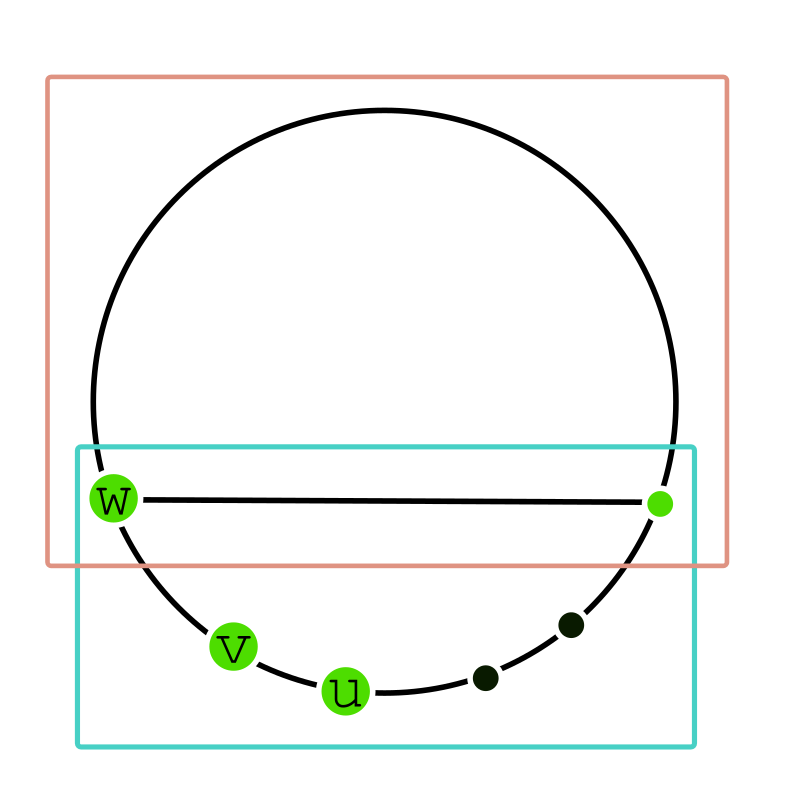
\includegraphics[scale=0.4]{images/5w1.png}
		\caption{Z wierzchołka $w$ wychodzi ,,cięciwa'' która dzieli graf na 2 podgrafy; tę część, która zawiera $v$ i $u$ kolorujemy z założenia indukcyjnego. Wtedy $w$ i wierzchołek którego on ,,dotyka'' dostają już jakiś określony kolor, wobec czego dla drugiego podgrafu również możemy zastosować założenie indukcyjne.}
	\end{figure}

	W sytuacji, gdy z $w$ nie ma takiej ,,cięciwy'', sytuacja robi się nieco śmieszniejsza, ale w sumie to nie bardzo. Oznacza to tyle, że jeśli $w$ się łączy z jakimś wierzchołkiem, to ma on listę o 5 kolorach (chyba, że są to wierzchołki ,,na zewnątrz'', które będą maksymalnie 2). W takim razie wykonujemy bardzo sprytny plan: tworzymy dwuelementowy podzbiór listy $w$, taki że nie ma on jedynego koloru na który możemy pokolorować $v$ (zawsze możemy taki podzbiór utworzyć). Teraz każdemu sąsiadowi $w$ z listą pięcioelementową przyporządkowujemy listę trójelementową, taką że nie ma ona żadnego z tamtych dwóch kolorów. Jak się to narysuje to się okaże, że graf zawierający wszystkie wierzchołki poza $w$, z tak zdefiniowanymi listami, możemy pokolorować z założenia indukcyjnego (rysunek powinien rozjaśnić dlaczego). Teraz dokładamy z powrotem $w$; zauważamy, że musi mieć on co najmniej 1 taki kolor, że możemy go pokolorować (bo miał pulę 2 kolorów których nie współdzielił z nikim poza potencjalnie jednym wierzchołkiem, ale jak ten wierzchołek dostał kolor to na pewno zostanie nam 1 wolny). As you might've already guessed, nie mam bladego pojęcia jak to sformalizować. Whoopsie. Ale tak poza tym to właśnie dowiedliśmy co mieliśmy dowieść.

	\begin{figure}[H]
		\centering
		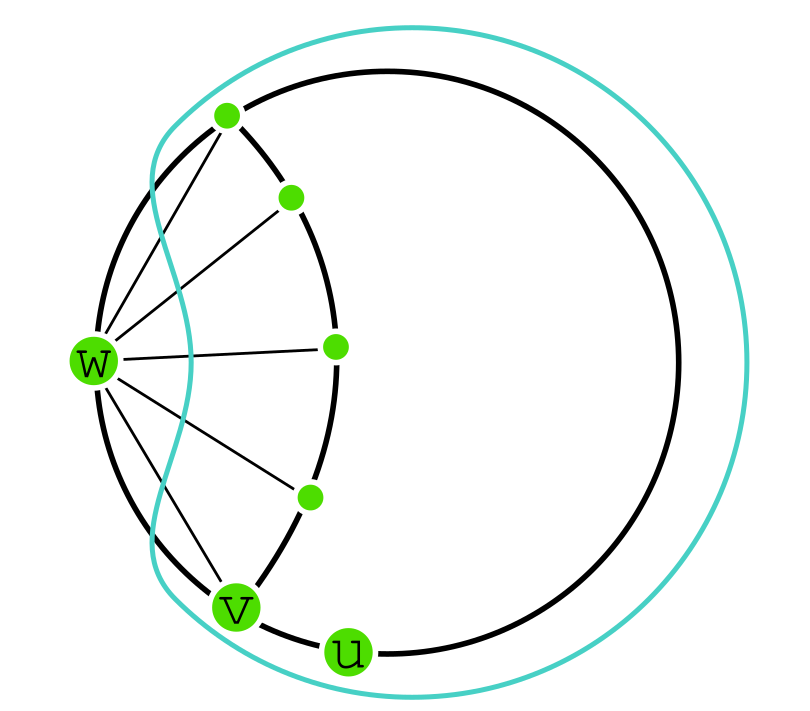
\includegraphics[scale=0.4]{images/5w2.png}
		\caption{Z $w$ nie wycohdzi żadna ,,cięciwa'', więc wszystkie wierzchołki z którymi się łączy mają listę długości 5 (poza $v$ i jednym wierzchołkiem na okręgu). Modyfikujemy listy wierzchołkom których on dotyka i które mają 5 elementów, a potem go wywalamy; wtedy te z którymi się łączył będą na zewnątrz, i z założenia indukcyjnego możemy je pokolorować. }
	\end{figure}
\end{proof}
